\let\negmedspace\undefined
\let\negthickspace\undefined
\documentclass[journal]{IEEEtran}
\usepackage[a5paper, margin=10mm, onecolumn]{geometry}
%\usepackage{lmodern} % Ensure lmodern is loaded for pdflatex
\usepackage{tfrupee} % Include tfrupee package

\setlength{\headheight}{1cm} % Set the height of the header box
\setlength{\headsep}{0mm}     % Set the distance between the header box and the top of the text

\usepackage{gvv-book}
\usepackage{gvv}
\usepackage{cite}
\usepackage{amsmath,amssymb,amsfonts,amsthm}
\usepackage{algorithmic}
\usepackage{graphicx}
\usepackage{textcomp}
\usepackage{xcolor}
\usepackage{txfonts}
\usepackage{listings}
\usepackage{enumitem}
\usepackage{mathtools}
\usepackage{gensymb}
\usepackage{comment}
\usepackage[breaklinks=true]{hyperref}
\usepackage{tkz-euclide} 
\usepackage{listings}
% \usepackage{gvv}                                        
\def\inputGnumericTable{}                                 
\usepackage[latin1]{inputenc}                                
\usepackage{color}                                            
\usepackage{array}                                            
\usepackage{longtable}                                       
\usepackage{calc}                                             
\usepackage{multirow}                                         
\usepackage{hhline}
\usepackage{pgf-pie}
\usepackage{ifthen}                                           
\usepackage{lscape}
\renewcommand{\thefigure}{\theenumi}
\renewcommand{\thetable}{\theenumi}
\setlength{\intextsep}{10pt} % Space between text and floats
\numberwithin{equation}{enumi}
\numberwithin{figure}{enumi}
\renewcommand{\thetable}{\theenumi}

% Marks the beginning of the document
\begin{document}
\bibliographystyle{IEEEtran}

\title{GateAssignment7}
\author{EE24BTECH11048-NITHIN.K} 
% \maketitle
% \newpage
% \bigskip
{\let\newpage\relax\maketitle}
\begin{enumerate}
\section{Q.1 - Q.5 carry one mark each}
%1
\item It is a common criticism that most of the academicians live in their \rule{1cm}{0.4pt}, so they are not aware of the real life challenges.
	\begin{enumerate}
		\item homes
		\item ivory towers
		\item glass palaces
		\item big flats
	\end{enumerate}
%2
\item His hunger for reading is insautible. He reads indiscriminately, He is most certainly a/an \rule{1cm}{0.4pt} reader.
	\begin{enumerate}
                \item all-round
                \item prcocious
                \item voracious
                \item wise
        \end{enumerate}
%3
\item Select the word that fits the analogy: \\
	Fuse : Fusion :: Use : \rule{1cm}{0.4pt}
	\begin{enumerate}
                \item all-round
                \item prcocious
                \item voracious
                \item wise
        \end{enumerate}
%4
\item If 0, 1, 2, ..., 7, 8, 9 are coded as O, P, Q,..., V, W, X, then 45 will be coded as \rule{1cm}{0.4pt}
	\begin{enumerate}         
                \item TS
                \item ST
                \item SS
                \item SU
        \end{enumerate}
%5
\item The sum of two positive numbers is 100. After subtracting 5 from each number, the product of the resulting numbers is 0. One of the original numbers is \rule{1cm}{0.4pt}.
	\begin{enumerate}
                \item 80       
                \item 85       
                \item 90       
                \item 95       
        \end{enumerate}
\section{Q6 - Q10 carry two marks each.}
%6
\item The American psychologist Howard Gardner expounds that human intelligence can be sub-categorised into multiple kinds, in such a way that individuals differ with respect to their relative competence in each kind. Based on this theory, modern educationists insist on prescribing multi-dimensional curriculum and evaluation parameters that enable development and assessment of multiple intelligences. \\
Which of the following statements can be inferred from the given text?
	\begin{enumerate}
                \item Howard Gardner insists that the teaching curriculum and evaluation needs to be multi-dimensional.
                \item Howard Gardner wants to develop and assess the theory of multiple intelligences.
                \item Modern educationists want to develop and assess the theory of multiple intelligences.
                \item Modern educationists insist that the teaching curriculum and evaluation needs to be multi-dimensional.
        \end{enumerate}
%7
\item Five friends P, Q, R, S and T went camping. At night, they had to sleep in a row inside the tent. P, Q and T refused to sleep next to R since he snored loudly. P and S wanted to avoid Q as he usually hugged people in sleep. \\
Assuming everyone was satisfied with the sleeping arrangements, what is the order in which they slept?
	\begin{enumerate}
                \item RSPTQ 
                \item SPRTQ
                \item QRSPT
                \item QTSPR
        \end{enumerate}
%8
\item Insert seven numbers between 2 and 34, such that the resulting sequence including 2 and 34 is an arithmetic progression. The sum of these inserted seven numbers is \rule{1cm}{0.4pt}.
	\begin{enumerate}
                \item 120
                \item 124
                \item 126
                \item 130
	\end{enumerate}
%9
\item The unit's place in $26591749^{110016}$ is \rule{1cm}{0.4pt}.
	\begin{enumerate}
		\item 1
                \item 3
                \item 6
                \item 9
	\end{enumerate}
%10
\item The total expenditure of a family, on different activities in a month, is shown in the pie-chart, The extra money spent on education as compared to transport $\brak{\text{in percent}}$ is \rule{1cm}{0.4pt}
	\begin{tikzpicture}
		\pie[
			radius = 2,
			text = legend,
			color = {blue!60, red!60, green!60, purple!60, cyan!60, orange!60, blue}
		]{
			5/Health (5\%),
			10/Transport (10\%),
			15/Household Items (15\%),
			15/Education (15\%),
			10/Leisure (10\%),
			20/House Rent (20\%),
			25/Others (25\%)
		}
	\end{tikzpicture}
	\begin{enumerate}
                \item 5
                \item 33.3
                \item 50
                \item 100
        \end{enumerate}
\section{Q1 - Q25 carryone mark each.}
%11
\item In the following partial differential equation, $\theta$ is a function of t and z, and D and K are functions of $\theta$ \\
	\begin{align*}
		D\brak{\theta}\frac{\partial^2\theta}{\partial z^2} + \frac{\partial K\brak{\theta}}{\partial z} - \frac{\partial \theta}{\partial t} = 0
	\end{align*}
	The above equation is
	\begin{enumerate}
                \item a second order linear equation
                \item a second degree linear equation
                \item a second order non-linear equation
                \item a second degree non-linear equation
        \end{enumerate}
%12
\item The value of $\lim_{x \to \infty}{\frac{x^2 - 5x + 4}{4x^2 + 2x}}$ is
	\begin{enumerate}    
                \item 0
		\item $\frac{1}{4}$
		\item $\frac{1}{2}$
                \item 1
        \end{enumerate}
%13
\item The true value of $\ln{\brak{2}}$ is 0.69. If the value of $\ln{\brak{2}}$ is obtained by linear interpolation between $\ln{\brak{1}}$ and $\ln{\brak{6}}$, the percentage of absolute error $\brak{\text{round off to the nearest integer}}$, is
	\begin{enumerate}                                                                              
                \item 35     
                \item 48                 
                \item 69                  
                \item 84                                 
        \end{enumerate}

\end{enumerate}
\end{document}
